\chapter{Data Collection} \label{chapter:datacollection}
In order to train a language model, a sufficiently large amount of data is needed. Since the model presented in this paper will be used for textual classification, the data must be available in written form.
Most of the data used for the report classification come from the FA laboratory. The laboratory has two sources to save information: an ontology which is the formalization of FA knowledge in a computer-friendly format, and the FA reports which comprise information that describes all diagnostic steps, results, and observations for a job analysis. These two resources would have a large enough amount of data to train the model. However, experiments with previous models indicated that these documents are too specific to serve as the sole data source for a model in the semiconductor domain. The content of the documents in the ontology and the FA reports contains too specific vocabulary and too little general vocabulary about electronics and semiconductors. Models which were trained only with this data did not have sufficient performance. For this reason, additional sources were sought to train the model more extensively.
This chapter starts by introducing the inddividual datasets and how they got collected before covering the data cleaning process to prepare it as an input for the PikaBERT model. 

\section{Data Sources}
The remaining dataset was created out of different data sources which got categorized in four datasets for an easier use in later experiments. The four datasets are: the \textit{FA ontology and reports}, the \textit{S2ORC Dataset}, the \textit{Infineon Dataset} and the \textit{Additional Dataset}. The following chapters introduce every dataset with its content, size and chatateristics.

\subsection{Failure Analysis Ontology and Reports}
\alert{The  FA  laboratory  stores  most  of  its  knowledge  as  free  texts, thus they might be ambiguous and cannot be processed by the software automatically. To avoid these issues, standard definitions of FA concepts used in the domain are required.  Moreover,  these  definitions  must  be stored  in  a  way that  they  can  be  used  by  both  engineers  and software tools alike. One  possible  solution  to  this  challenge  is  to  formalize  the knowledge about the FA domain as an ontology, a knowledge base  specifically  designed  to  store  terminological  definitions. This is the case for the FA laboratory, where an ontology is being  developed,  currently  storing  hundreds  of  failures,  tasks, tools, etc. The structure of an ontology includes classes, instances of these classes  and  properties.  Individuals  are  descriptions  of  real-world entities, like sample integrated circuits of a job or tools available  in  a  lab.  Classes  are  defining  parts  of  the  world  by summarizing  properties  of  a  collection  of  individuals.}

\alert{For training the classification models, we have considered the historical  data  of  the FA  laboratory.  These  reports  contain  a series  of  fields,  including  the  job  identification  number,  cus-tomer comment regarding the issues found in devices, an anal-ysis report describing applied methods, found physical defects, their  locations,  electrical  characterization,  and  other  details. Some of this data is structured and can be retrieved from corre-sponding databases. However, the essential parts relevant to the fault  identification  process  are  described  only  in  textual  form and, therefore, cannot be processed automatically.
Consider three samples taken from fault analysis reports of an FA  Laboratory  presented  in Error!  Reference  source  not found..  The  examples  show  selected  sentences  describing  the findings  of  an  engineer  and  the  labels  indicating  the  physical faults  and  their  electrical  signatures.  Both  types  of  labels  are organized in an ontology, which is a hierarchical structure rep-resenting a taxonomy of faults. This ontology allows for the de-velopment of software tools helping to label reports manually and working with the classification results. Along  with  the  job  summary,  the  reports  contain  a  series  of fields including, an identification number of the device, lists of tasks performed on the device, the images obtained by certain tools such as X-Ray,the  description of such images attached, etc. A subset of the reports also includesfault labels, both of the electrical signature of the faulty device and of the final physical failure.For the classification phase, these two faults are considered the target  output  while  the  job  summary  and  image  descriptions will constitute the input.}

\subsection{S2ORC Dataset}
The S2ORC Dataset was collected by the Allen Institute of Ar-tificial  Intelligence  and  it  has  a  corpus  of 81.1M  English-language academic papers from different domains. Around 40\% of the papers belong to the  biomedical field, as in Figure \ref{fig:domains}. The texts  got  extracted  from  PDFs  including  abstracts  and  inline mentions of citations.
The S2ORC-SciBERT is a SciBERT model which was further trained on the S2ORC dataset presented above. It got published simultaneously with the dataset itself from the same developers. Compared to SciBERT it has a wider corpus including 20 different  domains like  Computer  Science,  Mathematical  Science and Engineering which could be beneficial for the FA domain. However, it was also trained in Medical and Biology data which again could be a drawback for the model as with SciBERT.

\begin{figure}[H]
	\centering
	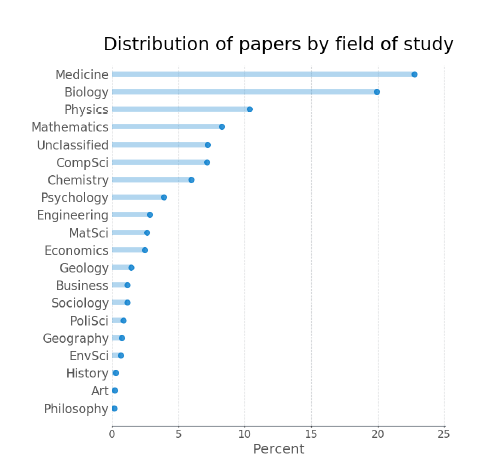
\includegraphics[width=0.6\textwidth]{figures/S2ORC_Domains.PNG}
	\caption{Different Domains in the S2ORC Dataset.}
	\label{fig:domains}
\end{figure}

\subsection{Infineon Dataset}
In addition, we created an Infineon Dataset comprising rele-vant textual data available on the company’s intranet. This dataset comprises 1.687 papers covering research topics and best-practices methods in the semiconductor domain. It was collected by employees and engineers of Infineon . Be-cause these papers got collected from engineers in different countries, we had to filter out non-English language papers. After filtering and extracting the raw text, we used approxi-mately 31.5MB of text data to create a dataset.

\subsection{Additional Data}
To increase the specificity of the training data for the FA domain, we also searched the Web for FA and electrical en-gineering papers. In this work we were using open search engines, like FreeFullPDF  and GoogleScholar , as well as specific sources, like IEEE, to collect the data. The text was extracted from the papers and converted into a text represen-tation. The resulting dataset comprises 12.31MB of raw text, where 2.33MB got collected from FreeFullPDF and Google-Scholar and the other 9.98MB from IEEE.

\section{Data Preprocessing}
For later usage during training, we combined the Infineon and the Additional Datasets in one. Moreover, since the biggest part of the S2ORC Dataset was medical and biomedical data, we filtered this dataset by using the FA ontology keywords, retaining only documents that comprise at least one keyword. The resulting filtered dataset contains approximately 542MB of raw text. For later discussions, we introduce the following abbreviations for the datasets:

\begin{itemize}
	\item \textbf{inf}: Infineon Dataset + Additional Dataset;
	\item \textbf{s2}: a part of the documents from S2ORC dataset fil-tered on keywords extracted from the ontology.
\end{itemize}

After finishing collecting the papers for the dataset, it was necessary to extract the raw text out of the documents. Therefore we got access to an text extractor API developed by Infineon collegues in Bangalore. The raw texts got extracted and UTF8 converted to be saved as excel sheets. \newline
Not all of the extracted text is important or useful for the dataset. To remove unuseful data, a notebook was created were the text got prepared before being cleaned. Authors, metadata about the images, tables and other not contiguous text was remoed. The resulting text got again saved as excel sheets.

\subsection{Data Cleaning}
To use the FA reports for AI purposes, their content must be pre-processed and cleaned to erase all data that can disrupt the training process. One of the biggest issues regarding the FA reports is the wide variety of styles in which they are written, as they come from several laboratories around the globe, some of them dealing with specific purposes, while others deal with a broader range of failures. It is also essential to consider that although all they are written in English, this is not a standard language as engineers are only rarely native speakers. \newline
The data cleaning process was the same for all datasets. A notebook was created were the excel sheets got loaded into dataframes. The methods used for cleaning the text are imported from the \alert{Natural Language Toolkit (nltk)} package which implements functions for normalization, stemming and lemmatization.
The following steps describe the procedure of text cleaning:

\begin{enumerate}
	\item \textbf{Remove Punctuations and Special Characters}: Punctuatins and special characters got removed inbetween and at the end of every sentence by using regular expressions because a language model is not able to interpret those characters. 
	\item \textbf{Remove Numbers}: The input got checked if it is a number or not. Also all words which are not strictly all letters got removed to avoid confusing the model.
	\item \textbf{Normalization}: After removing undesired words and characters, the entire text got normalized. This means that the resulting text contains only out of lowercased letters.
	\item \textbf{Remove Stop-Words}: The nltk package contains a collection of english stop-words like "and", "or", "but", "for" etc. Due to their low entropy they are useless for the training and therefore removed from the text.
	\item \textbf{Lemmatization}: Lemmatization considers the context of a word and converts it to its meaningful base form, which is called Lemma. For instance, lemmatizing the word "Caring" would return "Care". This has been done for the entire dataframe by iterating over the words.
	\item \textbf{Remove Empty Lines}: Due to the previous cleaning some cells or lines of the dataframe may be empty now and represented as NaN values in the dataframe. These NaN values have to be replaced with spaces, otherwise they will cause errors during further processing.
\end{enumerate}


\subsection{Dataset Formatting}
In comparison to traditional neural networks, BERT-based models are like a black box for the engineer. For training the model we used the so-called “transformer” class from \alert{Huggingface}.  The trainer method of the transformer class needs a model, a tokenizer and the training dataset as input. This input dataset needs to have a specific format and datatype otherwise the function would rise an error.  To do so the previous created dataframes got converted into dataframes of two cells, an index and a text cell. An example is shown in Table \ref{tab:format}.

\begin{table}[H]
	\centering
	\begin{tabular}{ll}
		\hline
		& \textbf{text}                                         \\ \hline
		0 & The following parameters are most often considered... \\ \hline
		1 & Nitrogen fertilization stands out as an important...  \\ \hline
	\end{tabular}
	\caption{Example of transformed dataframe shape}
	\label{tab:format}
\end{table}

The base class \textit{Dataset} from Huggingface implements a Dataset backed by an Apache Arrow table. This type of object can be created out of the dataframe just created with the following code:

\begin{minted}{python}
		train_dataset = Dataset.from_dict(df)
		datasets = datasets.DatasetDict({"train:" train_dataset})
\end{minted}

The dataset object allows to specify a training and a test dataset. Since training the language model is an unsupervised learning method, only the training dataset is needed. The resulting dataset objects were saved and could be loaded later for training.

\alert{Tokenizing dataset
split into blocks}